\documentclass[crop,tikz]{standalone}
%\usetikzlibrary{...}% tikz package already loaded by 'tikz' option

\usetikzlibrary{positioning}

 % times is deprecated - using a modern times clone instead
\usepackage{mathptmx}

\begin{document}

% Use monospace font (Latin Modern Typewriter) for all text.
% Source: https://tex.stackexchange.com/a/25251
%{\fontfamily{lmtt}\selectfont

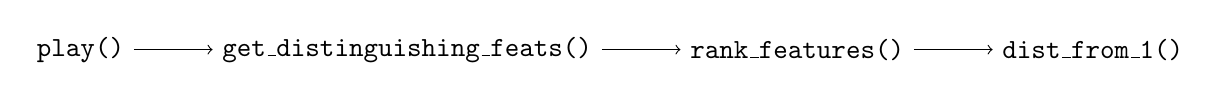
\begin{tikzpicture}


%\draw [->] (0,0) -- (10,10);

\node (play) at (0,0) {\texttt{play()}};

\node[right=1cm of play] (gdf) {\texttt{get\_distinguishing\_feats()}};
\node[right=1cm of gdf] (rf) {\texttt{rank\_features()}};
\node[right=1cm of rf] (df1) {\texttt{dist\_from\_1()}};

\draw [->] (play.east) -- (gdf.west);
\draw [->] (gdf.east) -- (rf.west);
\draw [->] (rf.east) -- (df1.west);

%\draw [->] (2) to [out=190, in=-10] (1);
	
\end{tikzpicture}

%}
	
\end{document}